% questions.tex —— 2011 年·全国大纲卷·文科 · 题目内容片段（无答案）
% 由 tools/generate_projects.py 依来源总账自 2011/2011_数学真题_全国大纲文_试题.md 生成，勿手改（改源 MD 后重跑）


\gkpart{数学}

\begin{gktip}
\textbf{来源说明}：本题面依据固定源 PDF 两页 A3 题面逐题转录，原卷印刷页码 657–658。固定源不附答案，答案和解析均由本库独立复算。

\textbf{图形说明}：第 20、22 题的原卷立体图或坐标图重绘为 TikZ/PGFPlots 矢量图。图形标记所指的 PNG 不随仓库保存。
\end{gktip}

\gkpart{一、选择题}

\begin{question}
\gkti{1}设集合 $U=\{1,2,3,4\}$，$M=\{1,2,3\}$，$N=\{2,3,4\}$，则 $\complement_U(M\cap N)=$\mbox{（　　）}

（A）$\{1,2\}$\quad（B）$\{2,3\}$\quad（C）$\{2,4\}$\quad（D）$\{1,4\}$

\end{question}
\begin{question}
\gkti{2}函数 $y=2\sqrt{x}$（$x\geq0$）的反函数为\mbox{（　　）}

（A）$y=\dfrac{x^2}{4}$（$x\in\mathbb R$）\quad（B）$y=\dfrac{x^2}{4}$（$x\geq0$）

（C）$y=4x^2$（$x\in\mathbb R$）\quad（D）$y=4x^2$（$x\geq0$）

\end{question}
\begin{question}
\gkti{3}设向量 $\boldsymbol a\text{、}\boldsymbol b$ 满足 $|\boldsymbol a|=|\boldsymbol b|=1$，$\boldsymbol a\cdot\boldsymbol b=-\dfrac12$，则 $|\boldsymbol a+2\boldsymbol b|=$\mbox{（　　）}

（A）$\sqrt2$\quad（B）$\sqrt3$\quad（C）$\sqrt5$\quad（D）$\sqrt7$

\end{question}
\begin{question}
\gkti{4}若变量 $x\text{、}y$ 满足约束条件

\nopagebreak[4]
\[
\begin{cases}
x+y\leq6,\\
x-3y\leq-2,\\
x\geq1,
\end{cases}
\]

则 $z=2x+3y$ 的最小值为\mbox{（　　）}

（A）$17$\quad（B）$14$\quad（C）$5$\quad（D）$3$

\end{question}
\begin{question}
\gkti{5}下面四个条件中，使 $a>b$ 成立的充分而不必要的条件是\mbox{（　　）}

（A）$a>b+1$\quad（B）$a>b-1$\quad（C）$a^2>b^2$\quad（D）$a^3>b^3$

\end{question}
\begin{question}
\gkti{6}设 $S_n$ 为等差数列 $\{a_n\}$ 的前 $n$ 项和，若 $a_1=1$，公差 $d=2$，$S_{k+2}-S_k=24$，则 $k=$\mbox{（　　）}

（A）$8$\quad（B）$7$\quad（C）$6$\quad（D）$5$

\end{question}
\begin{question}
\gkti{7}设函数 $f(x)=\cos\omega x$（$\omega>0$），将 $y=f(x)$ 的图象向右平移 $\dfrac\pi3$ 个单位长度后，所得的图象与原图象重合，则 $\omega$ 的最小值等于\mbox{（　　）}

（A）$\dfrac13$\quad（B）$3$\quad（C）$6$\quad（D）$9$

\end{question}
\begin{question}
\gkti{8}已知直二面角 $\alpha-l-\beta$，点 $A\in\alpha$，$AC\perp l$，$C$ 为垂足，点 $B\in\beta$，$BD\perp l$，$D$ 为垂足。若 $AB=2$，$AC=BD=1$，则 $CD=$\mbox{（　　）}

（A）$2$\quad（B）$\sqrt3$\quad（C）$\sqrt2$\quad（D）$1$

\end{question}
\begin{question}
\gkti{9}$4$ 位同学每人从甲、乙、丙 $3$ 门课程中选修 $1$ 门，则恰有 $2$ 人选修课程甲的不同选法共有\mbox{（　　）}

（A）$12$ 种\quad（B）$24$ 种\quad（C）$30$ 种\quad（D）$36$ 种

\end{question}
\begin{question}
\gkti{10}设 $f(x)$ 是周期为 $2$ 的奇函数，当 $0\leq x\leq1$ 时，$f(x)=2x(1-x)$，则 $f\left(-\dfrac52\right)=$\mbox{（　　）}

（A）$-\dfrac12$\quad（B）$-\dfrac14$\quad（C）$\dfrac14$\quad（D）$\dfrac12$

\end{question}
\begin{question}
\gkti{11}设两圆 $C_1\text{、}C_2$ 都和两坐标轴相切，且都过点 $(4,1)$，则两圆心的距离 $|C_1C_2|=$\mbox{（　　）}

（A）$4$\quad（B）$4\sqrt2$\quad（C）$8$\quad（D）$8\sqrt2$

\end{question}
\begin{question}
\gkti{12}已知平面 $\alpha$ 截一球面得圆 $M$，过圆心 $M$ 且与 $\alpha$ 成 $60^\circ$ 二面角的平面 $\beta$ 截该球面得圆 $N$。若该球面的半径为 $4$，圆 $M$ 的面积为 $4\pi$，则圆 $N$ 的面积为\mbox{（　　）}

（A）$7\pi$\quad（B）$9\pi$\quad（C）$11\pi$\quad（D）$13\pi$

\end{question}
\gkpart{二、填空题}

\begin{question}
\gkti{13}$(1-x)^{10}$ 的二项展开式中，$x$ 的系数与 $x^9$ 的系数之差为\gkblank{}。

\end{question}
\begin{question}
\gkti{14}已知 $\alpha\in\left(\pi,\dfrac{3\pi}{2}\right)$，$\tan\alpha=2$，则 $\cos\alpha=$\gkblank{}。

\end{question}
\begin{question}
\gkti{15}已知正方体 $ABCD-A_1B_1C_1D_1$ 中，$E$ 为 $C_1D_1$ 的中点，则异面直线 $AE$ 与 $BC$ 所成角的余弦值为\gkblank{}。

\end{question}
\begin{question}
\gkti{16}已知 $F_1\text{、}F_2$ 分别为双曲线 $C:\dfrac{x^2}{9}-\dfrac{y^2}{27}=1$ 的左、右焦点，点 $A\in C$，点 $M$ 的坐标为 $(2,0)$，$AM$ 为 $\angle F_1AF_2$ 的平分线，则 $|AF_2|=$\gkblank{}。

\end{question}
\gkpart{三、解答题}

\begin{question}
\gkti{17}设等比数列 $\{a_n\}$ 的前 $n$ 项和为 $S_n$，已知 $a_2=6$，$6a_1+a_3=30$，求 $a_n$ 和 $S_n$。

\end{question}
\begin{question}
\gkti{18}$\triangle ABC$ 的内角 $A\text{、}B\text{、}C$ 的对边分别为 $a\text{、}b\text{、}c$。已知

\nopagebreak[4]
\[
a\sin A+c\sin C-\sqrt2a\sin C=b\sin B.
\]

（1） 求 $B$；

（2） 若 $A=75^\circ$，$b=2$，求 $a\text{、}c$。

\end{question}
\begin{question}
\gkti{19}根据以往统计资料，某地车主购买甲种保险的概率为 $0.5$，购买乙种保险但不购买甲种保险的概率为 $0.3$。设各车主购买保险相互独立。

（1） 求该地 $1$ 位车主至少购买甲、乙两种保险中的 $1$ 种的概率；

（2） 求该地 $3$ 位车主中恰有 $1$ 位车主甲、乙两种保险都不购买的概率。

\Needspace{0.4\textheight}
\end{question}
\begin{question}
\gkti{20}如图，四棱锥 $S-ABCD$ 中，$AB\parallel CD$，$BC\perp CD$，侧面 $SAB$ 为等边三角形。$AB=BC=2$，$CD=SD=1$。
\nopagebreak[4]
\begin{center}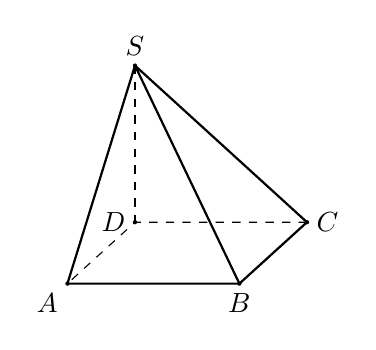
\begin{tikzpicture}[scale=.78,>=stealth]
\coordinate (A) at (0,0);
\coordinate (B) at (2.8,0);
\coordinate (C) at (3.9,1.0);
\coordinate (D) at (1.1,1.0);
\coordinate (S) at (1.1,3.55);
\draw[thick] (A)--(B)--(C);
\draw[dashed] (C)--(D)--(A);
\draw[thick] (S)--(A) (S)--(B) (S)--(C);
\draw[dashed] (S)--(D);
\fill (A) circle (1pt) node[below left] {$A$};
\fill (B) circle (1pt) node[below] {$B$};
\fill (C) circle (1pt) node[right] {$C$};
\fill (D) circle (1pt) node[left] {$D$};
\fill (S) circle (1pt) node[above] {$S$};
\end{tikzpicture}
\end{center}
\nopagebreak[4]
（1） 证明：$SD\perp$ 平面 $SAB$；

（2） 求 $AB$ 与平面 $SBC$ 所成角的大小。

\end{question}
\begin{question}
\gkti{21}已知函数 $f(x)=x^3+3ax^2+(3-6a)x+12a-4$（$a\in\mathbb R$）。

（1） 证明：曲线 $y=f(x)$ 在 $x=0$ 处的切线过点 $(2,2)$；

（2） 若 $f(x)$ 在 $x=x_0$ 处取得极小值，$x_0\in(1,3)$，求 $a$ 的取值范围。

\Needspace{0.4\textheight}
\end{question}
\begin{question}
\gkti{22}已知 $O$ 为坐标原点，$F$ 为椭圆 $C:x^2+\dfrac{y^2}{2}=1$ 在 $y$ 轴正半轴上的焦点，过 $F$ 且斜率为 $-\sqrt2$ 的直线 $l$ 与 $C$ 交于 $A\text{、}B$ 两点，点 $P$ 满足

\nopagebreak[4]
\[
\overrightarrow{OA}+\overrightarrow{OB}+\overrightarrow{OP}=\boldsymbol0.
\]
\nopagebreak[4]
\begin{center}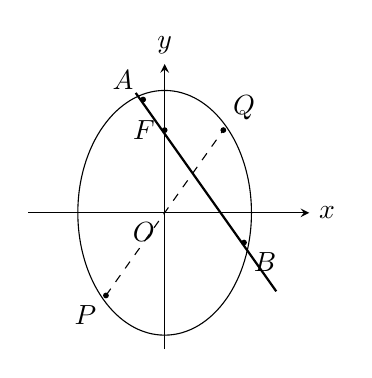
\begin{tikzpicture}[>=stealth,scale=1.05]
\draw[->] (-1.65,0)--(1.75,0) node[right] {$x$};
\draw[->] (0,-1.65)--(0,1.8) node[above] {$y$};
\draw (0,0) ellipse [x radius=1.05,y radius=1.48];
\draw[thick] (-.35,1.45)--(1.35,-.95);
\fill (-.26,1.37) circle (1pt) node[above left] {$A$};
\fill (.96,-.36) circle (1pt) node[below right] {$B$};
\fill (0,1) circle (1pt) node[left] {$F$};
\fill (-.71,-1) circle (1pt) node[below left] {$P$};
\fill (.71,1) circle (1pt) node[above right] {$Q$};
\draw[dashed] (-.71,-1)--(.71,1);
\node[below left] at (0,0) {$O$};
\end{tikzpicture}
\end{center}
\nopagebreak[4]
（1） 证明：点 $P$ 在 $C$ 上；

（2） 设点 $P$ 关于点 $O$ 的对称点为 $Q$，证明：$A\text{、}P\text{、}B\text{、}Q$ 四点在同一圆上。

\end{question}